\section{Additional Details to Err. Analysis \S\ref{sec:app_err_analysis}}
\label{appendix:err_analysis}

\subsection{Additional Case Study: Quantifiers}
\label{appendix:err_analysis_quantifier_case}

\begin{figure}[t]
\centering
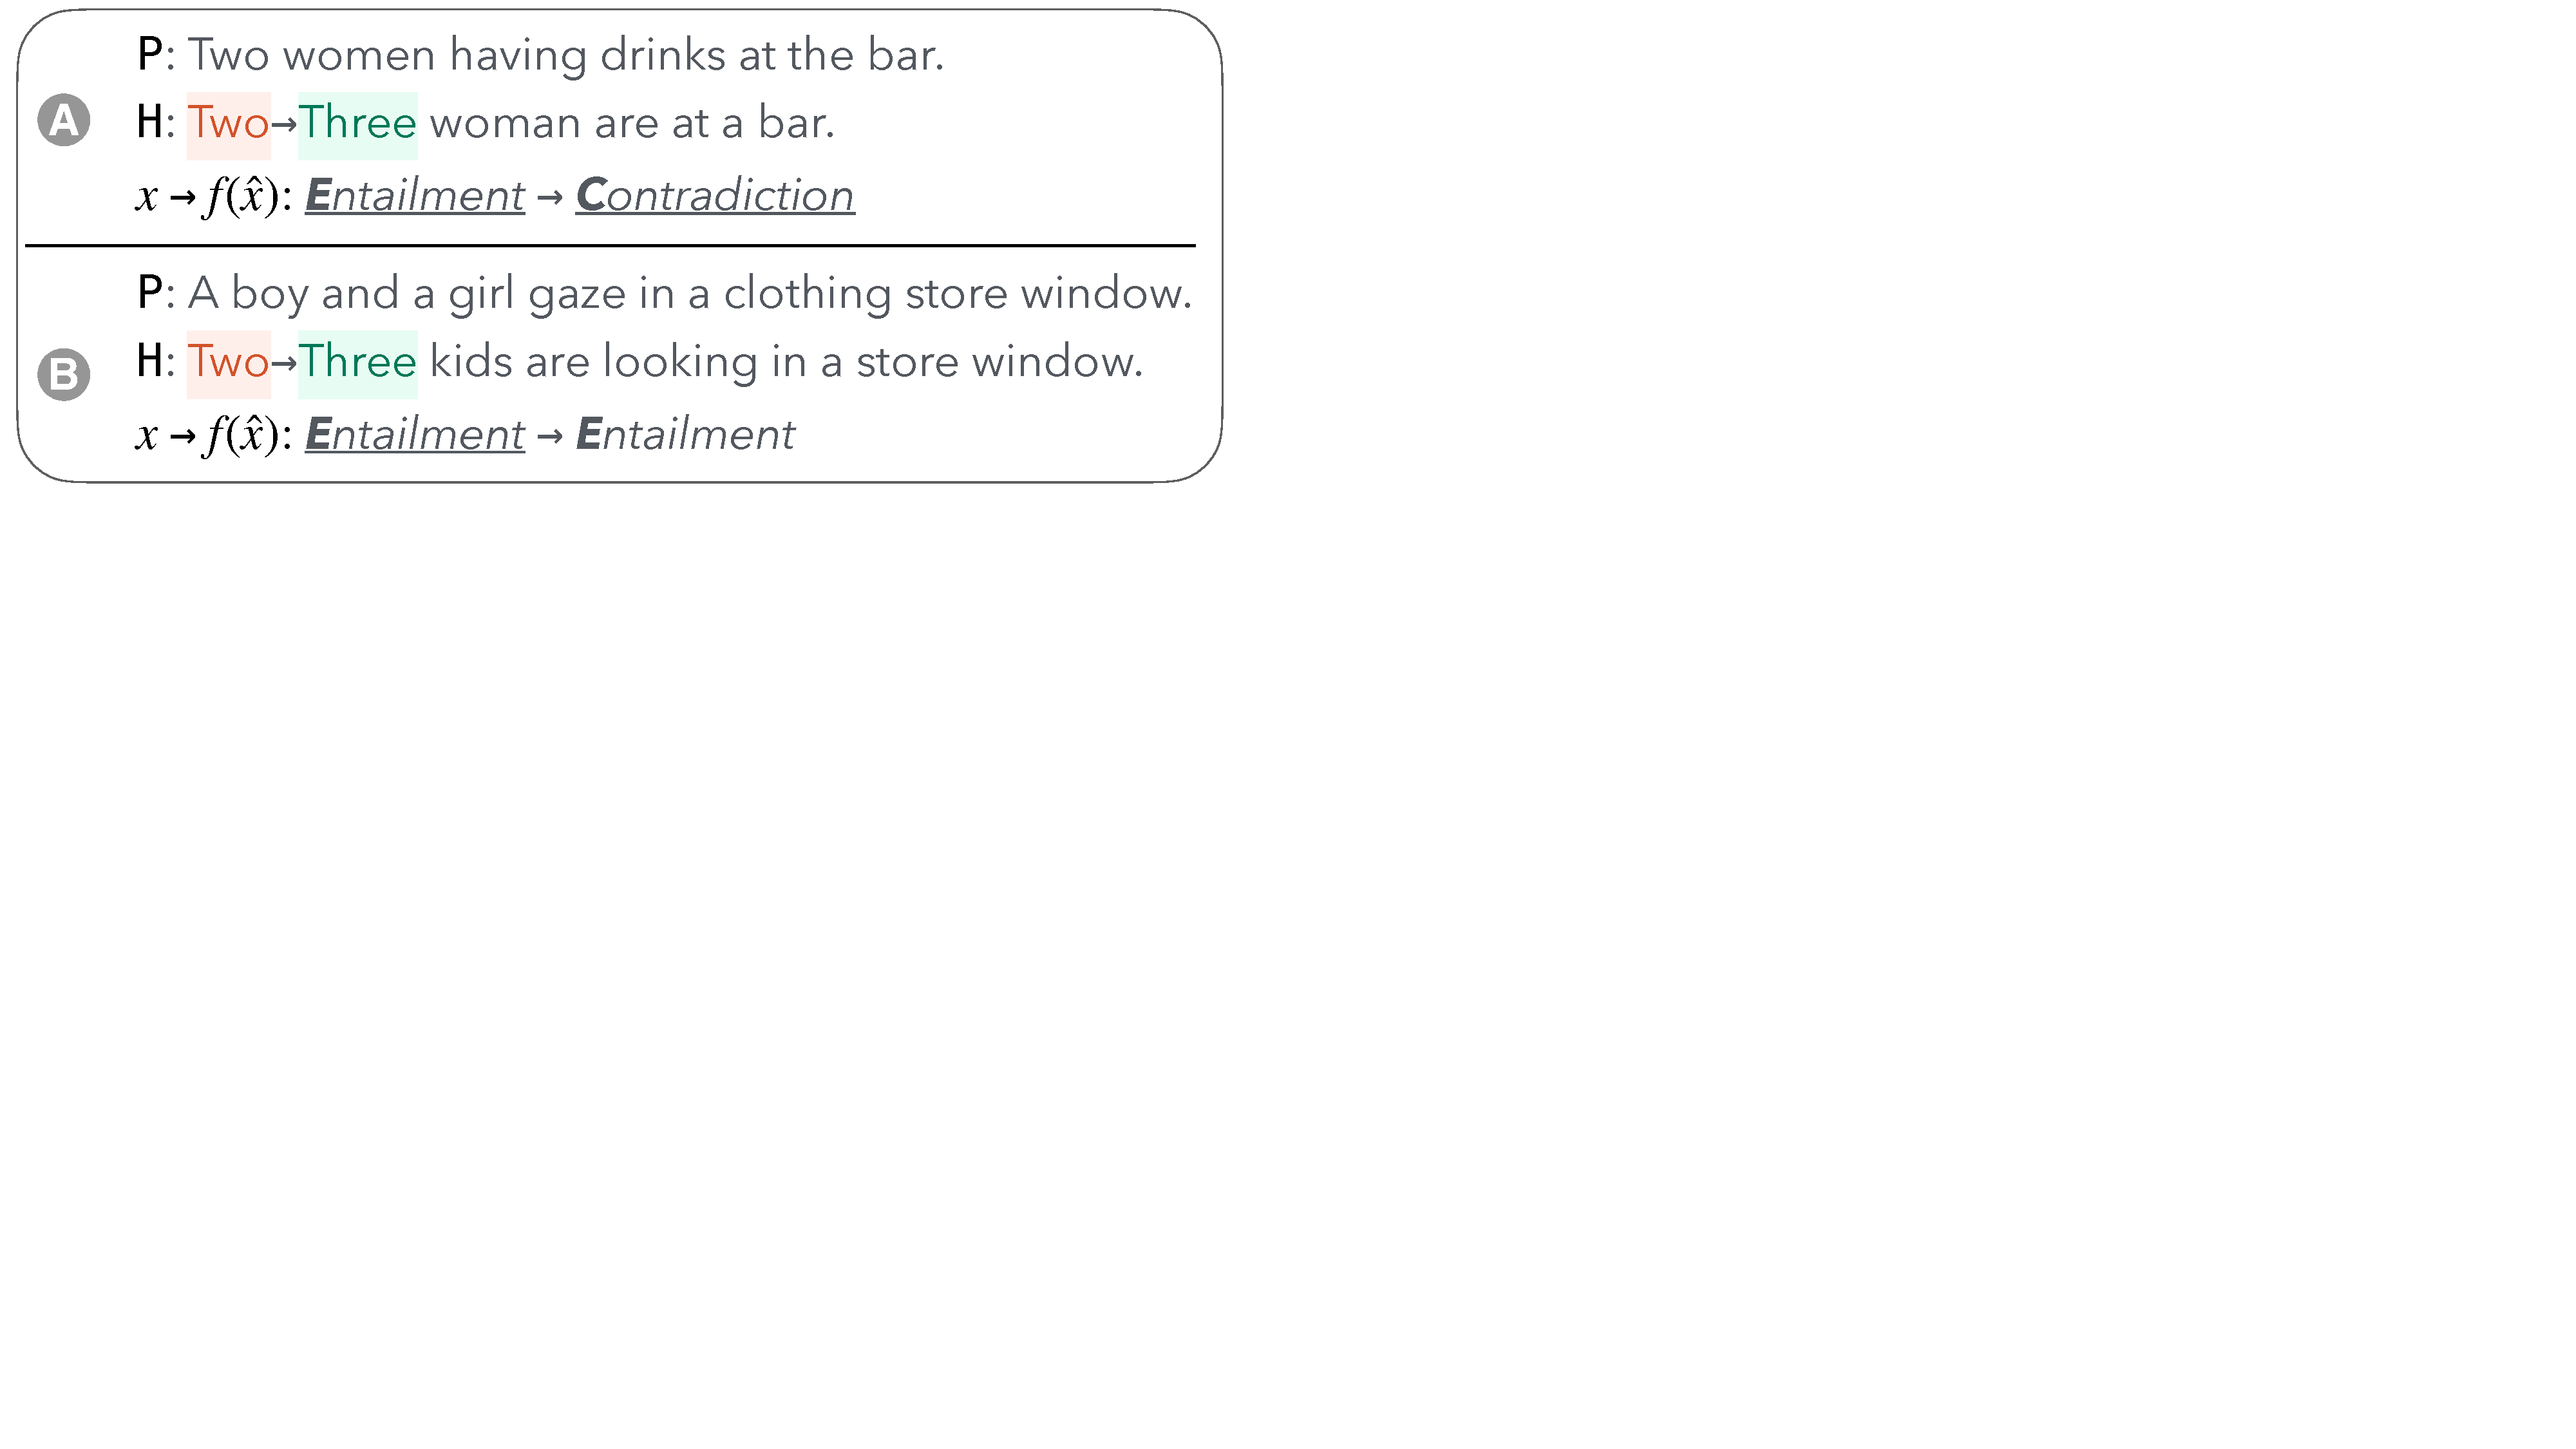
\includegraphics[trim={0 25.2cm 34.5cm 0cm},clip,width=1\columnwidth]{figures/err_analysis_two_three}
\vspace{-20pt}
\caption{
The \nli model cannot perform the actual counting when the exact number is missing from \emph{P}.
%In (B), it still predicts (the now incorrect) \emph{Entailment}.
}
\vspace{-10pt}
\label{fig:err_analysis_two_three}
\end{figure}


%\citet{gururangan2018annotation} also mentioned that one common strategy for creating NLI examples is to modify the numbers, suggesting that the model should have seen various examples related to numbers.

As a follow-up to Figure~\ref{fig:err_analysis_quantifier}, we slice the data to find \emph{entailement} instances that have numbers in the hypothesis sentence, and perturb their \ctrltag{quantifiers}.
The extracted templates show that the model does not perform actual counting. 
When changing one number to another (\swap{\texttt{NUM}}{\texttt{NUM}}), the model only flips the label in 64.7\% cases, while we would expect all cases to be like in Figure~\ref{fig:err_analysis_two_three}A.
Diving into the instances, the model seems easily confused when the explicit number is not in the premise. 
Indeed, when we filter the instance to only keep instances like in Figure~\ref{fig:err_analysis_two_three}B, the label flip rate of \swap{\texttt{NUM}}{\texttt{NUM}} further decreases to 30.2\%.

Further, the model only reacts to \emph{some} quantifier phrase modifiers. 
\addplus{at least} (\exinline{\add{at least} women are at a bar}) will always still result in \emph{entailment}, prediction, \addplus{only} and \swap{}{exactly} flip the predicted label to \emph{neutral} 90\% of the time (\exinline{\add{exactly} women are at a bar}), but the model only changes the prediction 52.6\% of the time when we add \addplus{more than} (\exinline{\add{more than} women are at a bar}).


\subsection{Representative Perturbation Templates}
\label{appendix:err_analysis_template}

Similar to \citet{wu2020tempura}, the process of finding representative perturbation patterns takes two steps:

\textbf{Extract template.}
For each $\xp$, we compare it with its $x$, and translate the perturbed spans into templates using different combinations of texts, lemmas, sparse and fine-grained part-of-speech tags.
We optionally include surrounding contexts determined by the parsing tree structure (tokens that share the same parents as the perturbed span).
For example, \exinline{is \add{not} reading} can result in templates $t$ as fine-grained as \swap{is reading}{is not reading}, or as sparse as \addplus{\texttt{PART}}.
Meanwhile, \exinline{are \add{not} playing} also translates to \addplus{\texttt{PART}} or \addplus{\texttt{not}}, but not \swap{is reading}{is not reading}.
As such, the $\xp$ and templates form a many-to-many relationship: each $\xp$ generates multiple templates, and each template covers a different group of $\xp$.

\textbf{Select Representative Templates.}
To find representative changes, we prefer (1) templates that cover a large number of $\xp$.
Meanwhile, to avoid overfitting to one instance (\eg extracting a template \swap{red}{\texttt{ADJ}} only because ``red'' is repeatedly perturbed in one $x$), we prefer (2) templates that perturb various unique $x$.
We also prefer (3) finer-grained templates, to avoid being unnecessarily abstract (\eg to avoid abstracting ``not'' when it is the only \texttt{PART} changed.)

%$\hat{\xset}_i$

With these intuitions, we form the template selection as a weighted set coverage problem.
We see the union of counterfactuals for each $x$, $\hat{\xset}$, as the entire set of elements.
Then, each template $t \in T = {t_1,...,t_m}$ represents a subset of $\hat{\xset}$ that contains a number of counterfactuals $|t|$.
We define the weight as $w(t) = g(t) / |t|_x$, where $|t|_x$ quantifies the unique original $x$ covered by $t$, and $g(t)$ represents the sparsity of $t$ (heuristically decreasing from \texttt{text} to \texttt{POS}).
This way, templates that are too abstract or too focused on a certain $x$ are penalized by having a high weight. 
We use a classic greedy algorithm~\cite{vazirani2013approximation} to select a subset of $T^* \subset T$, such that the aggregated coverage is maximized, and the weight is minimized.
